
\chapter{CTL下的遗忘理论的定义及其语义属性}\label{chapter03}
{\em 本章首先基于实现差分隐私的随机扰动原理,借鉴Shannon基本通信模型建立差分隐私通信模型。其次,从信息量化的角度,引入信息熵、联合熵、条件熵、互信息及失真函数等量化差分隐私保护前后的隐私信源熵、隐私泄露风险、数据效用。进一步,以此度量模型及方法为基础,针对多维关联属性的隐私量化问题,以关联性分析、关联依赖图模型、马尔可夫模型为理论基础,提出面向关联属性的信息熵度量方法。}

\section{引言}
数据密集型科学研究第四范式\cite{hey2009the},强调数据的重要性。可见,数据已成为支撑决策、人工智能、机器智能、挖掘分析的核心,尤其在普适计算模式下,数据正发挥着重要的价值。然而,随着数据流动,开放共享,用户隐私正在面临严峻的挑战。为解决隐私泄露问题,学术界与产业界开展了一系列积极而有意义的工作。其中,差分隐私(differential privacy,DP)\cite{dwork2006differential,dwork2006calibrating}因具有严格的数学理论支撑,逐步发展成为了隐私保护领域研究的热点。隐私保护的数据发布在差分隐私的诸多应用场景中占据着重要的地位。如在差分隐私的非交互式数据发布中,数据发布者旨在利用差分隐私噪声扰动发布原始数据集的净化版本,将其提供给数据使用者进行分析使用。数据发布势必涉及到隐私泄露与数据效用两方面,因此,对于隐私保护机制的研究,度量(Metrics)是应首要解决的基础性工作。当前,隐私缺乏定量化的定义\cite{Lifenghua16},隐私度量问题,特别是面向多维关联数据情景的隐私度量尚需要进一步研究\cite{ningbowu2019}。%例如,文献\cite{zhu2015correlated}指出由属性关联导致的数据隐私问题。
隐私度量是研究权衡隐私泄露与数据效用\cite{sankar2013utility,kalantari2018robust}解决方案的关键,同时也是隐私泄露风险分析及隐私量化评估的理论基础。 鉴于此,研究隐私度量问题具有重要的理论和实际应用价值。

在隐私度量\cite{alvim2012measuring,wagner2018technical,peng2016,xiongjinbo2018}的研究工作中,基于信息论的量化信息流\cite{smith2009on,boreale2015quantitative,alvim2011on,alvim2010differential}是一种被学者广泛接受的量化方法,受到了研究者的关注。所谓量化信息流就是使用信息熵、条件熵、互信息等概念来度量信息系统中信息流动,它也可以被用于量化一个信息系统中的信息泄露量。标准框架下的量化信息流是基于熵的信息量化,它是熵与信息测量\cite{renyi1961on}的发展。近年来,在解决差分隐私保护模型中隐私泄露与数据效用的权衡问题时,基于信息量化的方法奠定了信息论度量的基础\cite{mir2012information,alvim2011differential,wang2016on}。基于熵的度量是平均意义上的隐私泄露,它属于信息论模型下的差分隐私研究\cite{sarwate2014a}。相比于差分隐私模型\cite{dwork2006differential,dwork2006calibrating},前者的度量对数据分布做出了部分假设 ,而后者没有对数据分布做出任何假设。对数据分布的假设,考虑了数据先验分布的影响,捕捉到了在有些应用中敌手拥有关于数据的先验知识\cite{kalantari2018robust}。 基于上述的原因,从信息熵的角度研究隐私泄露风险与数据效用度量问题,对于隐私泄露风险量化分析和差分隐私最优化机制设计具有重要的理论意义。


目前,信息论方法的隐私度量应用于差分隐私研究,已取得了一定的研究成果。但是,随着系统应用的推进,尚存在一些问题需要进一步研究。当前相关研究工作中对`` 是''和``否''类型的二元对称信道研究较多,逐步发展到类别型数据且多以元组为离散型随机变量构建离散信源模型,较少考虑元组多维属性关联关系且缺少多类型属性组合方面的研究。为此,本文围绕差分隐私的应用,借鉴Shannon基本通信模型\cite{shannon1948a}(参见小节\ref{sec:shannon_comunication_system}介绍)构建差分隐私通信模型。为解决其中的隐私量化问题,本章以通信模型为基本出发点,基于信息熵、失真测度方法提出隐私泄露量化、数据效用量化的方法。然后,在面向多维属性关联的差分隐私数据发布应用中考虑了隐私泄露的信息熵量化方法。通过数据相关度分析,构建关联依赖图模型,进一步,利用图模型中的关键隐私泄露路径,提出面向关联属性的信息熵度量方法。结合数据处理不等式、费诺不等式,给出隐私泄露风险的界。由此,本章所提出的度量方法,奠定信息论方法研究的基础,亦可为隐私泄露风险评估提供基于信息论的理论支撑。

 \section{问题描述}
假设一个数据集$\mathcal{D}$由$n$条数据元组组成($|\mathcal{D}|=n$),其中每个元组包含有$k$个维度的属性,它们是有关特定个体的描述信息。例如,表~\ref{tab:origin} 所示数据集包含Age,Sex,Race等属性信息,医疗数据集包含姓名、血压、体重、疾病等属性。诸如此类的数据集可以表示为$n\times k$的矩阵,其中的行表示元组,列表示属性。本文中,假设离散型随机变量$X_i \in \mathcal{X}_i$表示属性集合$\bm{X}$中的第$i$个属性,$i=1,2,\cdots,k$,由此,$\bm{X}$是一个长度为$k$的随机变量序列,记作$\bm{X}=\{X_1,X_2,\cdots,X_i,\cdots,X_k\}$。进一步,令$|\mathcal{X}_i| = m_i$表示属性$X_i$取值域$\mathcal{X}_i$基数,则有$k$ 属性乘积空间$\mathcal{X}=\prod_{i=1}^{k}\mathcal{X}_i$,基数$m=\prod_{i=1}^{k} m_i$。数据集$\mathcal{D}$是可视为抽样于数据全集$\mathcal{X}^{n}$的多重集,也就是$\bm{X}^{n}$,表示随机变量序列$\bm{X}$的$n$次独立随机抽样。
 基于上述符号的表示,差分隐私非交互式数据发布表示为数据管理者利用发布机制发布原始数据集$\bm{X}^n$的近似副本$\hat{\bm{X}}^n$,以满足隐私保护与数据可用性需求。

目前,针对差分隐私的隐私度量工作中较少考虑多维属性之间存在的关联性依赖。但是,实际的应用场景中,有关个体的多维属性信息之间较少存在相互独立的情况,而且多维属性的相互关联可能会泄露个体的隐私信息。 例如,Age,Occupation与Marital-status的关联,医疗数据集中,血压和体重的相关性增加了疾病敏感信息泄露的风险。基于此,研究面向多维属性关联的隐私度量对于隐私保护机制设计是亟待解决、而又基础和关键的工作。由于数据集中具有多类别属性、相关联的数据结构形式,对其展开隐私度量研究面临的主要问题有:(1) 属性关联识别;(2) 属性相关性表示;(3) 关联属性的隐私度量。围绕这些问题的解决,本章中旨在基于关联分析方法结合信息熵分析属性关联图中隐私泄露关键路径,给出隐私信息熵度量方法。但是,多维混合数据类型给属性相关性分析带来困难,进而,细粒度考虑多属性相关性的隐私度量需要提出新的方法。

\section{差分隐私通信模型}\label{sec:communication_model_of_dp}
差分隐私的标准定义形式\ref{def:dp},约束随机化函数$Q$在输出空间$S$上满足概率性输出的$\epsilon$-不可区分性。本质上,实现差分隐私的随机化函数$Q$ 与\ref{sec:shannon_comunication_system}小节Shannon信息论噪声信道数学模型$\left \{X~Q(\hat{X}|X)~\hat{X}\right \}$的转移条件概率矩阵$q(\hat{x}|x)$ 表示具有相似之处。以此为基础,差分隐私接受输入原始数据$X^n$,噪声扰动输出净化合成数据集$\hat{X}^n$,从信息论的角度借鉴通信系统模型\ref{sec:shannon_comunication_system}建立差分隐私的基本通信模型。其中,原始数据假设为隐私信源$\bm{X}$、 输出数据为信宿$\hat{\bm{X}}$,差分隐私随机化机制抽象为噪声信道$Q$,如图\ref{fig:chapter04-communication_of_dp}描绘了差分隐私随机化映射$Q$的通信模型。

 \begin{figure}[htbp]
 	\centering
 	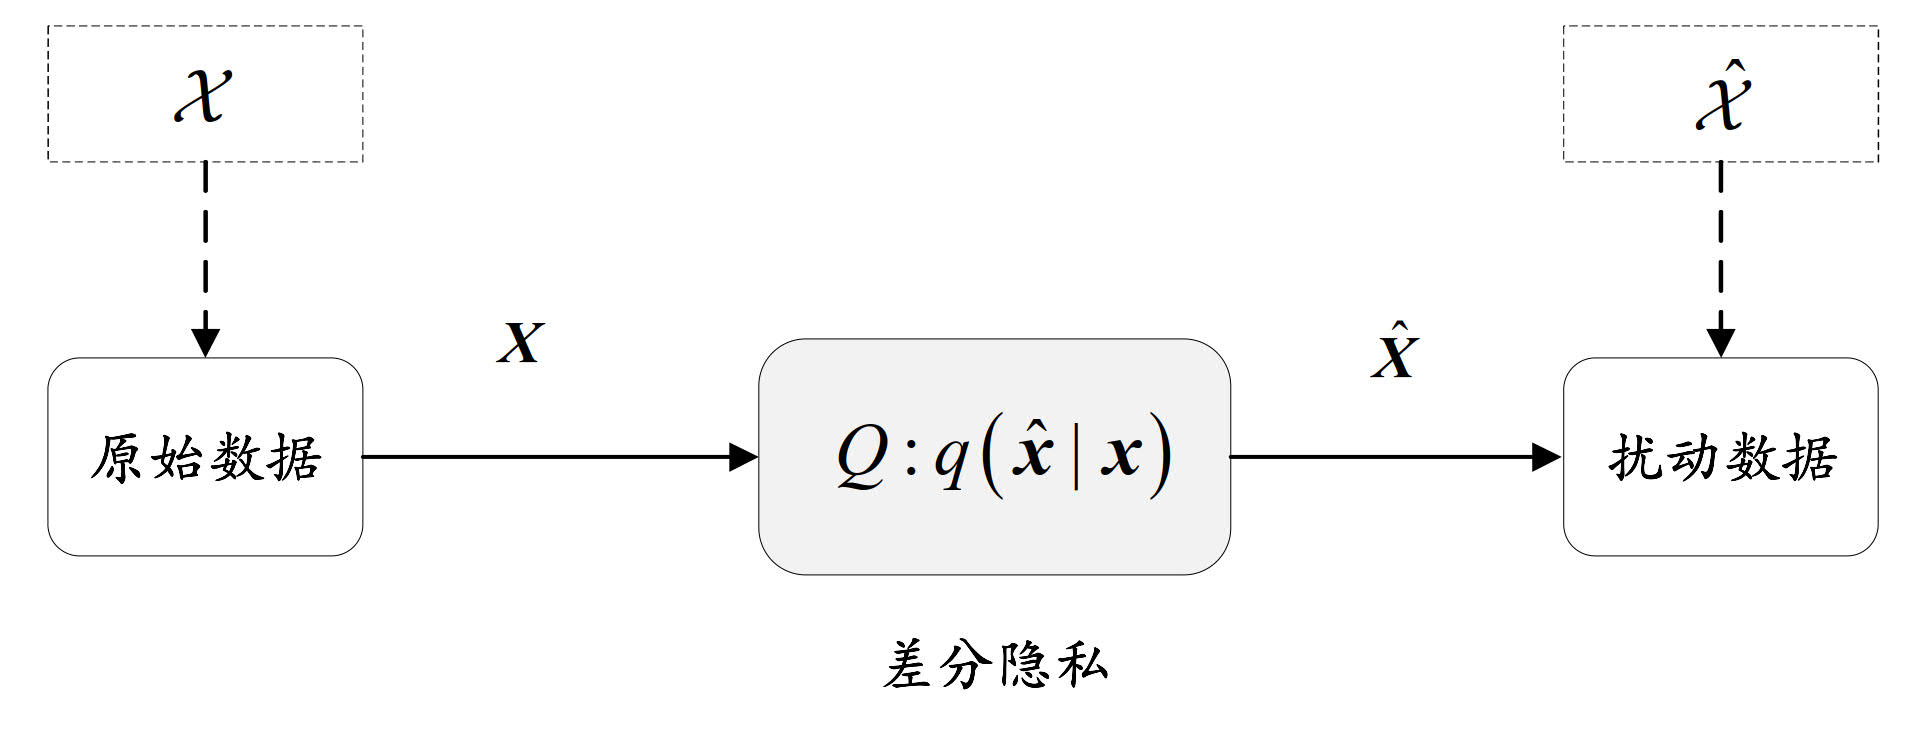
\includegraphics[width = 0.65\linewidth]{./figures/chapter04_1.jpg}
 	\caption{差分隐私的基本通信模型}
 	\label{fig:chapter04-communication_of_dp}
 \end{figure}


  以上述信道模型$\left \{\bm{X}~Q(\hat{\bm{X}}|\bm{X})~\hat{\bm{X}}\right \}$为基础,本章给出差分隐私的一个等价定义。不失一般性,假设输入数据$\bm{x}$取值于离散型字母表$\bm{x}\in \mathcal{X}$,输出数据$\hat{\bm{x}}$来源于字母表$\hat{\bm{x}} \in \hat{\mathcal{X}}$,如此,差分隐私形成一个噪声信道$Q$,随机概率性映射$Q:\mathcal{X}\rightarrow \hat{\mathcal{X}}$。基于这样的信道模型假设,差分隐私可以被正式的定义为如下的表述形式\cite{alvim2011differential}。

 \begin{definition}\label{def:dp_channel}假设$\mathcal{X}$和$\hat{\mathcal{X}}$为离散有限集合,分别表示原始数据输入和扰动数据输出字母表。如果一个随机化概率性映射$Q:\mathcal{X}\rightarrow \hat{\mathcal{X}}$满足$\epsilon$-差分隐私,当且仅当条件概率$q(\cdot|\cdot)$满足
 	\begin{equation}
 		q(\hat{\bm{x}}|\bm{x})\leq \exp(\epsilon) \cdot q(\hat{\bm{x}}|\bm{x}') \quad  \forall \hat{\bm{x}} \in \hat{\mathcal{X}}, \bm{x},\bm{x}' \in \mathcal{X}, \bm{x}\sim \bm{x}'
 	\end{equation}
 其中,隐私参数$\epsilon^* = \min\left\{\epsilon:q(\hat{\bm{x}}|\bm{x})\leq \exp(\epsilon) \cdot q(\hat{\bm{x}}|\bm{x}')\right\}$。
 \end{definition}

基于上述定义\ref{def:dp_channel},差分隐私直接表述为噪声信道条件概率矩阵的特性,采用$\log \frac{q(\hat{\bm{x}}|\bm{x})}{q(\hat{\bm{x}}|\bm{x}')}$量化差分隐私保护强度。对此定义,给出以下两点解释说明。首先,上述差分隐私定义提供了数据分布独立的隐私保障,$\epsilon$-隐私度量仅依赖于信道条件概率$q(\hat{\bm{x}}|\bm{x})$。其次,对于有限的$\epsilon > 0$,概率矩阵中相同输出元素$\hat{\bm{x}}$的条件概率不可能同时存在零和非零的概率。除此之外,$\bm{X}$与$\hat{\bm{X}}$之间的相关度测量给定$\hat{\bm{X}}$时有关$\bm{X}$的隐私泄露信息量,$\bm{X}$与$\hat{\bm{X}}$ 之间的失真程度$d(\bm{X},\hat{\bm{X}})$测量数据质量损失。以此为基础,本章中\ref{sec:information_theoretic_metrics}节给出差分隐私机制的信息熵度量模型及方法。



\section{隐私与效用度量}\label{sec:information_theoretic_metrics}
基于上述\ref{sec:communication_model_of_dp}节介绍的差分隐私通信模型,接下来,从量化信息流的角度,本章利用信息熵、互信息、失真函数等概念分别给出隐私信源、隐私泄露风险、数据效用的度量方法,为后续研究奠定度量基础。

\subsection{隐私信源熵}
信息熵的定义\ref{def:entropy}描述了隐私信源的不确定程度,它刻画了消除隐私信源不确定度平均需要的信息量,由此,信息熵也可表达隐私信源的平均隐私信息量。针对单属性情景,将其视为离散随机变量$X_i$,具有$m_i$个不同的元素$\alpha_u,u=1,2,\cdots,m_i$。由此,隐私信源数学模型定义为
\begin{equation}
\begin{pmatrix}
X_i\\
P(X_i)
\end{pmatrix}=\begin{Bmatrix}
\alpha_{1}, & \alpha_{2}, & \cdots, & \alpha_{u}, & \cdots,  & \alpha_{m_i}\\
p(\alpha_{1}),& p(\alpha_{2}), & \cdots, & p(\alpha_{u}), & \cdots, & p(\alpha_{m_i})
\end{Bmatrix}
\end{equation}
$0 \leq p(\alpha_u) \leq 1$,$\sum_{u=1}^{m_i}p(\alpha_u)=1$,则隐私信源熵$H(X_i)=-\sum_{u=1}^{m_i}p(\alpha_u) \log p(\alpha_u)$。
进一步,推广应用到~$k$~维属性情景时,概率空间为数据集域值空间的$m$种所有可能组合。信源$\bm{X}$的概率模型表示为~$k$~维属性联合概率分布
\begin{equation}
	\begin{pmatrix}
		\bm{X}\\
		P(\bm{X})
	\end{pmatrix}=\begin{Bmatrix}
		\beta_{1}, & \beta_{2}, & \cdots,  & \beta_{v}, & \cdots,  & \beta_{m}\\
		p(\beta_{1}),& p(\beta_{2}), & \cdots, & p(\beta_{v}), & \cdots, & p(\beta_{m})
	\end{Bmatrix}
\end{equation}
$0 \leq p(\beta_v) \leq 1$,$\sum_{v=1}^{m}p(\beta_v)=1 (v=1,2,\cdots,m)$。$\beta_v \in \{\alpha_{u_1},\alpha_{u_2},\cdots,\alpha_{u_i}\},1\leq i \leq k, 1\leq u_i \leq m_i$是一个$k$元组,其中元组的第$i$个分量是随机变量$X_i$的某个具体取值$\alpha_u$。基于此,$k$维属性的联合信源熵表示为随机变量序列的联合熵,记作$H(\bm{X}) = H(X_1,X_2,\cdots,X_k)$。依据熵的链式法则(定理\ref{theorm:multi_joint_entropy_}中公式\ref{eq:joint_entropy}),则有多属性联合信源熵
\begin{alignat}{2}
	H(\bm{X}) & = H(X_1,X_2,\cdots,X_k) \\
	& = -\sum_{x_1,x_2,\cdots, x_k} p(x_1,x_2,\cdots, x_k)\log p(x_1,x_2,\cdots, x_k)\\
	& = -\sum_{x_1,x_2,\cdots, x_k} p(x_1,x_2,\cdots, x_k)\log \prod_{i=1}^{k}p(x_i|x_{i-1},\cdots,x_1)\\
	& = \sum_{i=1}^{k}H(X_i|X_{i-1},\cdots,X_1)\label{eq:chapter03-7}
\end{alignat}



事实上,多维属性之间相互独立是属性关联的一种特例情况,属性独立时的联合概率$P(\bm{X}=\bm{x})=\prod_{i=1}^{k} P(X_i=x_i)$,条件概率$p(x_i|x_{i-1},\cdots,x_1)=p(x_i)$成立。由公式~\ref{eq:chapter03-7}易知,元组属性相互独立时,$k$维属性联合$\bm{X}=\{X_1,X_2,\cdots,X_i,\cdots,X_k\}$的信源熵$H(\bm{X})$满足可加性,表示为
\begin{equation}
	H(\bm{X})=\sum_{i=1}^{k}H(X_i)
\end{equation}
多维属性联合信源熵$H(\bm{X})$量化了个体隐私信息的不确定度,从元组整体上对隐私属性信息进行度量。如果数据集元组独立同分布的抽样于数据取值字母表集合,则可以使用
离散平稳无记忆信源的$n$次扩展信源模型表达扩展后的隐私信源模型,记作$\bm{X}^{n}$表示信源$\bm{X}$的$n$次扩展。信源$\bm{X}^{n}$数学模型表示为

\begin{equation}
	\begin{pmatrix}
		\bm{X}^n\\
		P(\bm{X}^n)
	\end{pmatrix}=\begin{Bmatrix}
		\vec{x}_{1}, & \vec{x}_{2}, & \cdots,  & \vec{x}_{i}, & \cdots , & \vec{x}_{m^n}\\
		p(\vec{x}_{1}),& p(\vec{x}_{2}), & \cdots,& p(\vec{x}_{i}), & \cdots, & p(\vec{x}_{m^n})
	\end{Bmatrix}
\end{equation}
其中的$p(\vec{x}_{i})=\prod_{j=1}^{n}p(x_{i_j})$表示$n$个符号消息序列的联合概率。由此,根据熵的定义\ref{def:entropy},离散无记忆信源$X$的$n$次扩展信源熵$H(X^n)$可表示为
\begin{alignat}{2}
	H(\bm{X}^{n})  &=  -\sum_{X^n}p(\vec{x}) \log p(\vec{x}) \\
	& =  -\sum_{X^n}\left(\prod_{j=1}^{n}p(x_{i_j})\log \prod_{j=1}^{n}p(x_{i_j})\right)\\
	& = -n\sum_{i=1}^{m}\sum_{j=1}^{n}p(x_{i_j}) \log p(x_{i_j}) \\
	& = nH(X_1,X_2,\cdots,X_k)\\
	& =n\sum_{i=1}^{k}H(X_i|X_{i-1},\cdots,X_1)
\end{alignat}

%通常非独立的情景下,联合熵的计算依据熵的链式法则(定理\ref{theorm:multi_joint_entropy_}中公式\ref{eq:joint_entropy}),在此不再过多的赘述。
隐私信源熵度量了原始隐私信息的平均不确定量,表达了信源消除不确定度平均所需要的比特数,刻画了隐私信源特征。
\subsection{隐私泄露风险}
本章中考虑隐私攻击者或敌手可以观察到信道输出结果,在这样的敌手模型下,隐私攻击者观察噪声信道输出$\hat{\bm{X}}^n$后对信源消息$\bm{X}^n$仍具有的不确定度可以使用条件熵$H(\bm{X}^n|\hat{\bm{X}}^n)$度量。首先,$n$次扩展信源$\bm{X}^n$经差分隐私构成离散无记忆信道$\{\bm{X}~Q(\hat{\bm{X}}|\bm{X})~\hat{\bm{X}}\}$的$n$次扩展信道模型,条件概率满足$q(\bm{X}^{n}|\hat{\bm{X}}^n)=\prod_{i=1}^{n}q(\bm{X}^i|\hat{\bm{X}}^i)$。由此采用条件熵定义的平均隐私熵$E$满足
\begin{equation}
	E=\frac{1}{n}H(\bm{X}^{n}|\hat{\bm{X}}^n) = -\frac{1}{n}\mathbb{E} \log q(\bm{X}^{n}|\hat{\bm{X}}^n)= -\frac{1}{n}\mathbb{E} \log \prod_{i=1}^{n}q(\bm{X}^i|\hat{\bm{X}}^i)
\end{equation}
故有,
\begin{equation}
	E= -\frac{1}{n}\sum_{i=1}^{n}\mathbb{E} \log q(\bm{X}^i|\hat{\bm{X}}^i) = \frac{1}{n}\sum_{i=1}^{n}H(\bm{X}^i|\hat{\bm{X}}^i)
\end{equation}
鉴于此,得到平均隐私熵
\begin{equation}
	E=  -\frac{1}{n}\sum_{i=1}^{n}\left(\sum_{\bm{x} \in \mathcal{X}}\sum_{\hat{\bm{x}} \in \hat{\mathcal{X}}}p(\bm{x},\hat{\bm{x}})\log q(\bm{x}|\hat{\bm{x}})\right)
\end{equation}

依据熵与互信息的关系(参见\ref{sec:entropty_mutual_information}小节),互信息量可用于度量$\hat{\bm{X}}^{n}$含有信源$\bm{X}^n$的信息量。本质上,条件熵与互信息的度量可以平等对待,本章中利用互信息$I(\bm{X}^{n};\hat{\bm{X}}^{n})$的含义定义隐私泄露风险函数$L(\bm{X}^{n},\hat{\bm{X}}^{n})$量化平均意义上的隐私泄露量
\begin{alignat}{2}
	L(\bm{X}^{n},\hat{\bm{X}}^{n}) & = \frac{1}{n}I\left(\bm{X}^{n};\hat{\bm{X}}^{n}\right)\\
	& = \frac{1}{n}\left(H(\bm{X}^{n})-H(\bm{X}^{n}|\hat{\bm{X}}^{n})\right)\label{eq:privacy_leakage_risk}\\
	&=\frac{1}{n}\left (nH(\bm{X})-\sum_{\bm{X},\hat{\bm{X}}}H(\bm{X}|\hat{\bm{X}})\right )\\
	& \leq H(\bm{X})-\frac{1}{n}\sum_{\bm{X},\hat{\bm{X}}}H(\bm{X}|\hat{\bm{X}})
\end{alignat}
借鉴离散无记忆信道$n$次扩展信道的重要结论,信道输出变量仅依赖于输入变量与其它变量条件独立,则有$	L(\bm{X}^{n},\hat{\bm{X}}^{n})=\frac{1}{n}\sum_{\bm{X},\hat{\bm{X}}}I(\bm{X};\hat{\bm{X}})=I(\bm{X};\hat{\bm{X}})$。互信息隐私泄露风险是平均意义上的隐私泄露度量,它可以被解释成为一个敌手在平均意义上需要的比特数,用于完全的识别出特定的个体数据\cite{oya2017back}。由上述公式\ref{eq:privacy_leakage_risk} 可知,固定信源分布,$L(\bm{X}^{n},\hat{\bm{X}}^{n})$与$H(\bm{X}^{n}|\hat{\bm{X}}^{n})$负相关。由于互信息是信源分布和条件概率分布的函数,该测量在信息论的差分隐私模型中得到了广泛的应用。

\subsection{数据效用量化}

为解决损失压缩问题,Shannon信息论引入了失真测量函数,量化随机变量和它的表示之间的失真程度\cite{cover2006elements}。受此启发,本章中数据效用度量差分隐私噪声信道输出合成数据集副本与原始数据集的失真距离,也就是数据质量。采用非负的失真函数$d(\bm{X}^{n},\hat{\bm{X}}^{n})\rightarrow \mathbb{R}^{n}$量化原始输入与扰动输出的失真程度,测量发布数据的可用性,定义期望失真
\begin{equation}\label{eq:chapter03-ED}
\mathbb{E}\left[d(\bm{X},\hat{\bm{X}})\right]=\sum_{\bm{x},\hat{\bm{x}}}p(\bm{x})q(\hat{\bm{x}}|\bm{x})d(\bm{x},\hat{\bm{x}})
\end{equation}
量化平均意义上的失真程度。失真测量中的汉明失真($d(\bm{x},\hat{\bm{x}})=1,\bm{x} \neq \hat{\bm{x}}; d(\bm{x},\hat{\bm{x}})=0, \bm{x}=\hat{\bm{x}}$)是一种严格的失真测量,称为示性函数,具有灵敏度高的特点,对于具有明确含义的类别型数据特别有意义。由汉明失真可以得到一个误差概率失真\cite{cover2006elements}
\begin{equation}\label{eq:expected_hamming_distortion}
	\mathbb{E}\left[d(\bm{X},\hat{\bm{X}})\right]={\rm Pr}\left\{\bm{X} \neq \hat{\bm{X}}\right\}
\end{equation}
%度量合成数据集与原始输入数据集序列的失真程度,衡量集的整体可用性。由于数据集混合数值型与类别型属性,通常总是假设$\mathcal{X}=\mathcal{\hat{X}}$。


%度量输入与输出序列对应位置不同符号数目, 其优势在于无论差分隐私机制输入与输出符号改变多小,基于汉明失真的效用度量能够维持较高的灵敏度,尤其对于类别型数据很有意义。此外,平均意义的汉明失真度量发布合成数据集与原始数据集的平均失真程度,定义发布合成数据集的期望汉明失真函数


其中${\rm Pr}\left\{\bm{X} \neq \hat{\bm{X}}\right\}$表示$\bm{X}$与$\hat{\bm{X}}$之间的误差概率。因失真的度量方法比较直观、且具有降低计算复杂性的优势\cite{oya2017back},它已经被应用在差分隐私的相关研究工作中量化数据效用(如文献\mycite{andres2013geo,kalantari2018robust,sarwate2014a,wang2016on})。文中基于期望汉明失真,从隐私信源分布、噪声信道条件概率、扰动输出数据的方面量化差分隐私保护系统平均情况下的数据失真程度,实现发布合成数据与原始数据之间的效用度量。
\section{关联属性隐私度量模型及方法}
上述\ref{sec:information_theoretic_metrics}小节,讨论了信息论方法量化隐私与效用的一般性理论。接下来,将上述结论推广到多维属性关联的差分隐私应用场景,以下从关联属性相关度量化、关联依赖图模型表达、数据关联的隐私度量方面展开叙述。
\subsection{关联属性相关度}\label{sec:correlation_inditifity}
数据集$\mathcal{D}$中元组有$k$个属性,由随机变量序列$\bm{X}=\{X_1,X_2,\cdots,X_i,\cdots,X_k\}(1 \leq i \leq k)$表示个体数据信息。通常情况下,$k$ 个属性并不相互独立,而是存在数据的关联。如果存在$l(1 <k)$ 个属性与$X_i$属性关联,则称它们是一个关联属性组,记作$\bm{R}_i=\{X_i,X_j \in \bm{X}\mid$ 属性集合中与属性$X_i$具有关联关系的属性$X_j\}$。

为了表达多维属性的关联,首先给出属性关联的相关度分析方法。利用相关性分析方法对属性集合$\bm{X}$中属性依次分析属性对$(X_i;X_j)$,$X_i \neq X_j$ 之间的相关度。假设$m_i$,$m_j$分别表示属性$X_i$,$X_j$的基数,$z_{ij}$表示属性$X_i$与$X_j$ 的二维联合频率矩阵中第$i$个元素和第$j$个元素的频率统计值。则基于上述符号表示,可以得到一个具有$m_i \times m_j$个元素的二维属性联合频率表,如下表\ref{tab:table_frquence_4.1}所示。

\begin{table*}[htb]
\small
\centering
\caption{二维属性联合频率表}
\label{tab:table_frquence_4.1}
\begin{tabular}{p{2cm}p{2cm}p{2cm}p{2cm}p{2cm}}
\hline\noalign{\smallskip}
&$X_j(1)$  &$X_j(2)$ &$\cdots$ & $X_j(m_j)$\\
\noalign{\smallskip}\hline\noalign{\smallskip}
$X_i(1)$ & $z_{11}$ & $z_{12}$ & $\cdots$ & $z_{1m_j}$\\
$X_i(2)$ & $z_{21}$ & $z_{22}$ & $\cdots$ & $z_{2m_j}$\\
$\vdots$ & $\vdots$ & $\vdots$ & $\vdots$ & $\vdots$\\
$X_i(m_i)$ & $z_{m_i1}$ & $z_{m_i2}$ & $\cdots$ & $z_{m_im_j}$\\
\noalign{\smallskip}\hline
\end{tabular}
\end{table*}

基于上述表\ref{tab:table_frquence_4.1},属性联合概率分布$P_{ij}=P(X_i=i,X_j=j)$,表示$X_i$属性域中第$i$个值和属性$X_j$ 属性域中第$j$个值同时发生的事件频率。进一步,$P_{i\cdot}$和$P_{\cdot j}$分别表示$X_i$和$X_j$的边缘概率分布,则有,$P_{i\cdot}=\sum_{j}P_{ij}$和$P_{\cdot j}=\sum_{i}P_{ij}$。此外,在相关性分析方法上,Shanon互信息量化了两个随机变量之间的信息相关性,是一种相关性分析方法。对比与其它统计学上的相关性分析方法,互信息可以克服线性和非线性关系的局限性\cite{liangjy2016,reshef2011detecting},在敏感度方面具有较好的优势。基于此,本章中利用互信息方法测量属性集合中任意两者之间的相关性。正式的,定义属性$X_i$,$X_j$之间的相关度为互信息量,根据互信息量的计算公式
\begin{equation}\label{eq:mi_correlation}
	I(X_i;X_j)=\sum_{i=1}^{m_i}\sum_{j=1}^{m_j}P_{ij}\log \frac{P_{ij}}{P_{i \cdot}\cdot P_{\cdot j}}
\end{equation}
进行属性对的相关度分析,为后续多属性关联的属性依赖图表达奠定基础。接下来,给出具体的依赖图构建细节描述。
\subsection{关联属性图模型}
数据集$\mathcal{D}$中属性对$(X_i,X_j),1\leq i,j \leq k$的相关度表达出了元组属性的近似关联依赖强度,依据公式\ref{eq:mi_correlation}计算属性间的互信息量可以得到任意两属性的相关度。结合互信息性质,首先给出以下定理,为下文依赖图处理奠定基础。


\begin{theorem}\label{theorem:chapter04_2.1}
	对于相互关联的属性对$(X_i,X_j)$,互信息量$I(X_i;X_j)$表达为相关度$\theta_{ij}$,$I(X_j;X_i)$表达为相关度$\theta_{ji}$,则有$\theta_{ij}$,$\theta_{ji} \geq 0$ 和 $\theta_{ij}=\theta_{ji}$。
\end{theorem}

上述定理\ref{theorem:chapter04_2.1}的证明利用互信息的对称性、非负性质,本文中不再过多赘述其证明过程。

\begin{corollary}\label{cor:chapter04_2.2}如果属性$X_i$,$X_j$之间的相关度$\theta_{ij}=\theta_{ji}=0$,则属性对$(X_i,X_j)$相互独立,即是$X_i$,$X_j$之间满足$P(X_i,X_j)=P(X_i)P(X_j)$。
\end{corollary}

针对元组属性集合$\bm{X}=\{X_1,X_2,\cdots,X_k\}$,利用互信息的相关性分析方法,得到$(X_i,X_j),1\leq i,j \leq k$之间的相关度。首先,定义关联依赖图$G(V,E)$表达属性关联依赖,其中,$V$表示图中的顶点集合,$E$表示属性之间关联依赖构成的边集合。由于互信息的对称性,$X_i$与$X_j$之间的边$X_i-X_j$是无向边,则图$G(V,E)$是无向图。为表达属性对$(X_i,X_j)$之间的关联依赖强度$\theta_{ij}$,定义顶点$X_i$到$X_j$的边$X_i-X_j$的权值构成带权无向图$G$。其次,利用图的标准表示方法,对数据集属性关联依赖图$G(V,E)$采用邻接矩阵的形式表示,以下给出带权无向图$G$的邻接矩阵$\Theta$定义。


\begin{definition}带权无向图$G$中的顶点序列化$1,2,\cdots,k$,图$G$的邻接矩阵表示为$k$阶矩阵$\Theta$,矩阵元素$\Theta[i][j]$满足
	
	\begin{equation}
		\Theta[i][j]=
		\begin{cases}
			0 & \text{$\theta_{ij} < \omega $}\\ % 需要强制换行
			\theta_{ij} & \text{$\theta_{ij} \geq \omega $}
		\end{cases}
		\text{$1 \leq i,j \leq k$}
	\end{equation}
其中,$\theta_{ij}$为$X_i$与$X_j$的相关度$I(X_i;X_j)$,$\omega$为设置伪相关的阈值门限参数。
\end{definition}

依据推论\ref{cor:chapter04_2.2},邻接矩阵$\Theta$中元素$\Theta[i][j]=0$表示无相关的独立属性$X_i$和$X_j$。基于上述\ref{sec:correlation_inditifity}节中的数据集相关属性分析方法,可以用上述相关度邻接矩阵$\Theta$表达出属性集合中的相关属性关联程度。结合互信息量的对称性、非负性特点\cite{shannon1948a},易知邻接矩阵$\Theta$是对角线元素为$0$的对称矩阵。


\begin{algorithm}[htb]
 \small
 \setstretch{1.2}
\caption{ 图$G$的邻接矩阵$\Theta$生成算法}
\label{alg:gen_Theta}
\begin{algorithmic}[1]
\REQUIRE ~~\\
	\begin{tabular}[t]{p{1mm}l}
	 $\mathcal{D}$&:数据集\\
	 $\bm{X}$&:属性$\{X_1,X_2,\cdots,X_i,\cdots,X_k\}$\\
	 $k$&:属性维度\\
	 $\omega$&:阈值参数
	\end{tabular}
	\ENSURE ~~\\
	\begin{tabular}[t]{p{1mm}l}
	$\Theta$&: 图$G$邻接矩阵
	\end{tabular}
\STATE 初始化图$G$邻接矩阵$\Theta$元素
\FOR{$i=1,\cdots,k$}
\FOR{$j=1,\cdots,i$}
\STATE 设置矩阵元素$\Theta_{ij}=\Theta_{ji}=0$~/*初始属性独立*/
\ENDFOR
\ENDFOR
\FOR{$i=1,\cdots,k$}
\STATE 设置$V=\bm{X}\setminus\{X_i\}$实现属性的依次分析
\FOR{对于$V$中的每一个属性$X_j$}
\STATE 利用数据集$\mathcal{D}$,依据互信息量公式\ref{eq:mi_correlation}计算$\theta_{ij}=I(X_i;X_j)$
\STATE /*过滤伪相关或弱相关的属性关系*/
\IF{$\theta_{ij} \geq \omega$}
\STATE 赋值邻接矩阵元素$\Theta_{ij}=\Theta_{ji}=0$
\ENDIF
\ENDFOR
\ENDFOR
\RETURN 图$G$的邻接矩阵$\Theta$
\end{algorithmic}
\end{algorithm}


算法\ref{alg:gen_Theta}中的伪代码描述了通过数据集关联属性相关度分析,生成带权无向图$G$邻接矩阵$\Theta$的过程。以下给出算法计算过程分析,首先,算法初始化邻接矩阵$\Theta$中元素$\Theta_{ij}=0$对所有的$ 1\leq i,j \leq k$,矩阵初始化状态表示数据集中属性之间相互独立(算法\ref{alg:gen_Theta}中$1 \sim 6$行)。其次,算法依次计算属性对$(X_i,X_j)$之间的互信息量$I(X_i;X_j)$,并根据阈值$\omega$过滤属性边$X_i-X_j$集合,设置图$G$中无向边的权值$\theta_{ij}$(算法\ref{alg:gen_Theta}中的$7 \sim 16$行)。 最后,算法输出属性关联带权无向图$G$的邻接矩阵$\Theta$。

\begin{remark}
{\em 上述算法\textup{\ref{alg:gen_Theta}}的计算开销主要是计算互信息的关联属性相关度,算法的复杂度是数据集属性维度规模$k$的函数,计算输出属性关联带权无向图$G$邻接矩阵$\Theta$的计算时间复杂度为$O(k^2)$,是一个多项式时间算法。此外,在空间复杂度方面,图$G$的邻接矩阵$\Theta$是满足主对角线元素$\Theta_{ij}=0$的$k$阶对称矩阵,采用矩阵的压缩存储可将$\Theta$存储到$\frac{k(k-1)}{2}$个单位存储空间。}
\end{remark}
\subsection{关联属性隐私度量}
基于以上分析,本小节中阐述利用关联依赖图模型度量关联属性隐私的方法。首先,在属性依赖图$G(V,E)$中考虑和敏感属性$X_h$,取值域基数$|\mathcal{X}_h|=m_h$,具有直接相连边的属性组$\bm{R}_{h}$。 假设关联属性组$\bm{R}_{h}$是数据发布者和其它用户已知的非敏感数据知识,隐私获取者可通过其它途径获取的辅助知识。针对此,考虑敏感属性$X_h$通过差分隐私信道编码随机输出$\hat{X}_h$的情况,则有$X_h$与$\hat{X}_h$之间构成的信道特性,表示为条件概率依赖关系$Q:\mathcal{X}_h\rightarrow\hat{\mathcal{X}}_h$。基于上文\ref{sec:communication_model_of_dp}小节中的差分隐私通信模型的信道数学模型,扰动输出的数据边缘分布仅依赖于条件概率分布和敏感属性$X_h$的分布,条件独立于关联属性组$\bm{R}_{h}$,则有
\begin{theorem} \label{theorem:chapter04_markov_graph}
	无向图$G=(V,E)$中,敏感属性顶点$X_h \in V$及其关联属性组$\bm{R}_h\subset V$,与差分隐私信道$X_h \xrightarrow{Q} \hat{X}_{h}$输出$\hat{X}_{h}$之间的概率性依赖构成马尔可夫隐私链$\bm{R}_{h}\rightarrow X_{h}\rightarrow\hat{X}_{h}$的关系。
\end{theorem}

上述定理\ref{theorem:chapter04_markov_graph}结合差分隐私数据处理阐述了图$G$中由关联而存在的马尔可夫隐私链关系。其中,关联属性组$\bm{R}_{h}$的联合概率是初始的概率分布,条件概率$P(X_{h}|\bm{R}_{h})$表达了关联属性组对敏感属性$X_h$的影响,刻画了$X_h$与$\bm{R}_h$之间的条件性依赖。基于此,考虑差分隐私机制$Q$具有条件转移概率$Q(\hat{X}_h|X_h)$的形式,从信息论的角度使用条件概率$q(\hat{x}_{h}^{j}|x_{h}^{i})$表示隐私敏感属性$X_h$取值域$\mathcal{X}_h$ 中第~$i$~个原子符号转移输出域$\mathcal{\hat{X}}_h$中第~$j$~个原子符号的概率。由此,根据定义\ref{def:dp_channel},差分隐私机制$Q$满足概率不可区分条件的最小预算参数$\epsilon^*$,
则有
\begin{equation}\label{eq:epsilon_2.10}
	\epsilon^{*}=\min_{q(\hat{x}_h|x_h)}\log \left(\frac {q(\hat{x}_{h}^{j}|x_{h}^{i})}{q(\hat{x}_{h}^{j}|x_{h}^{t})}\right) \qquad \forall x_h^i \neq x_h^t, x_h^i , x_h^t\in \mathcal{X}_h
\end{equation}

基于上述表达,给出信息熵的度量与分析。首先,隐私泄露风险计算公式\ref{eq:privacy_leakage_risk}是隐私攻击者观察扰动输出$\hat{X}_h$后获得有关敏感信息$X_h$的互信息量$I(\hat{X}_h;X_h)$。结合数据关联的隐私链关系,依据数据处理不等式定义\ref{def:dataprocessinginequality},则有关联属性组$\bm{R}_h$ 与敏感属性$X_h$之间的互信息量$I(\bm{R}_h;X_h)$满足$I(\bm{R}_h;\hat{X}_h) \leq I(\bm{R}_h;X_h)$,即是隐私关联属性组$R_h$和$\hat{X}_h$的隐私信息上界。当$X_h$和$\hat{X}_h$之间相互独立时,类似于通信系统中断,$I(\bm{R}_h;\hat{X}_h)$信息量达到最小值$0$。其次,对于满足期望失真度$D={\rm Pr}\{X_h \neq \hat{X}_h\}$的差分隐私试验信道,互信息隐私泄露量$I(X_h;\hat{X}_h)$满足
\begin{alignat}{2}
	I(X_h;\hat{X}_h) & =H(X_h)-H(X_h|\hat{X}_h) \label{eq:entropty_2.10}\\
	 & = H(X_h)-H(D)-D\log(m_h-1) \label{eq:2.11}
\end{alignat}

对于属性域$\mathcal{X}_h = \hat{\mathcal{X}}_h$时,依据费诺不等式的推论\ref{cor:chapter02-1}易证公式\ref{eq:2.11}。基于互信息的隐私泄露度量依赖于差分隐私噪声信道转移概率$Q(\hat{X}_h|X_h)$和数据先验概率分布。此外,基于失真的数据效用度量公式\ref{eq:expected_hamming_distortion}演变为信道的误差概率,则有
$D={\rm Pr}\{X_h\neq \hat{X}_h\}$。误差概率量化了差分隐私噪声信道输入原始数据$X_h$与扰动输出数据$\hat{X}_h$之间的期望汉明失真度。由此可见,数据效用度量表达了差分隐私概率信道的统计特性。
\section{实验与分析}
本章中实验部分利用Java编程实现,采用机器学习Adult$\footnote{http://archive.ics.uci.edu/ml/}$公开数据集,在i5处理器,4G内存,安装Win10 X64系统的个人PC上运行。如表\ref{tab:origin}~所示数据集属性结构,选取其中的Age、Workclass、Education、Marital-status、Occupation、Race、Sex 七个属性,分别记作$X_1,X_2,\cdots,X_7$。Adult 数据集中混合数值型和类别型属性,共包含有$30718$个数据元组记录,属性域值空间基数$m =7902720$。本节中基于\ref{sec:correlation_inditifity} 节的方法,统计原始样本数据集中二维属性对$(X_i,X_j)$的频数,计算频率意义上的列联表。依据大数定律,当样本容量$n$趋于无穷大时,二维属性联合频率近似于二维属性联合概率分布。以此为基础,利用互信息量分析属性的相关度,生成属性的相关度矩阵$\Theta$,如下表\ref{tab:attributes_dependency_degree}所示。
\begin{table*}[htb]
	%\scriptsize
    \small
	\centering
	\caption{属性相关度矩阵}
	\label{tab:attributes_dependency_degree}
	\begin{tabular}{p{1.2cm}p{1.2cm}p{1.2cm}p{1.2cm}p{1.2cm}p{1.2cm}p{1.2cm}p{1.2cm}}
		\hline\noalign{\smallskip}
		&$X_1$  &$X_2$ &$X_3$ & $X_4$& $X_5$& $X_6$& $X_7$\\
		\noalign{\smallskip}\hline\noalign{\smallskip}
		$X_1$ & $0$&	$0.0548$&	$0.1537$&	$0.3353$&	$0.0936$&	$0.0097$&	$0.0119$\\
		$X_2$ & $0.0548$&	$0$&	$0.0429$&	$0.0272$&	$0.1668$&	$0.0102$&	$0.0168$\\
		$X_3$ & $0.1537$&	$0.0429$&	$0$&	$0.0308$&	$0.3352$&	$0.0147$&	$0.0063$\\
		$X_4$ & $0.3353$&	$0.0272$&	$0.0308$&	$0$&	$0.0764$&	$0.0185$&	$0.1653$\\
		$X_5$ & $0.0936$&	$0.1668$&	$0.3352$&	$0.0764$&	$0$&	$0.019$&	$0.1488$\\
		$X_6$ & $0.0097$&	$0.0102$&	$0.0147$&	$0.0185$&	$0.019$&	$0$&	$0.0095$\\
		$X_7$ & $0.0119$&	$0.0168$&	$0.0063$&	$0.1653$&	$0.1488$&	$0.0095$&	$0$\\
		\noalign{\smallskip}\hline
	\end{tabular}
\end{table*}

基于表\ref{tab:attributes_dependency_degree}所示的属性相关度,设定阈值参数$\omega=0.05$过滤多属性之间由噪声导致的伪相关和弱相关现象,生成属性关联依赖图$G$。如下图\ref{Fig:attributes_dependence_graph}所示,数据集属性为图$G$的顶点,相关度为$G$的无向边权值。从图\ref{Fig:attributes_dependence_graph}中分析,属性关联依赖图有效地表达了属性之间的关联信息。
\begin{figure}[htbp]
	\centering
	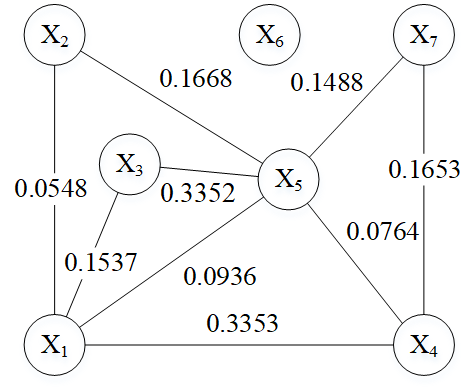
\includegraphics[width=3.0in]{./figures/chapter03/Figure1.png}
	\caption{属性关联依赖图}
	\label{Fig:attributes_dependence_graph}
\end{figure}

基于实验中的数据集,假设Marital-status($X_4$)为隐私敏感属性,则图$G$中与顶点$X_4$存在路径则构成隐私链,和$X_4$存在直接相连的边的属性构成关联属性组$\{X_1,X_5,X_7\}$。为和上文陈述保持一致,使用随机变量$X_h$表示隐私敏感属性$X_4$,$\bm{R}_h$表示和$X_4$存在关联的属性组。基于此利用本章中的信息熵方法量化关联属性的隐私泄露量。首先,基于样本观测数据统计关联属性组$\bm{R}_h$的联合概率分布,计算关联属性组联合信息熵$H(\bm{R}_h)=9.6712$ 。其次,计算敏感属性与关联属性组的联合信息熵$H(\bm{R}_hX_h) =10.8469$。由于原始数据集中的Marital-status为类别型数据,包含有七种不同的类别型取值,将其视为信源字母表空间,即域值。然后,利用敏感属性的概率分布计算隐私信源熵$H(X_h)=1.82$。进一步,基于熵与互信息的关系,计算得到互信息量$I(\bm{R}_h;X_h)=0.6442$,表示由属性关联导致的隐私敏感属性的信息泄露量。另外,条件熵$H(X_h|\bm{R}_h)$度量有关$X_h$仍具有的隐私不确定度,即$H(X_h)-I(\bm{R}_h;X_h)=1.1758$。

基于马尔可夫模型的隐私泄露链$\bm{R}_{h}\rightarrow X_{h}\rightarrow\hat{X}_{h}$关系,从信息论信道转移矩阵$Q(\hat{x}_h|x_h)$ 的角度构成马尔可夫状态转移矩阵。基于此,结合实验中的数据和数据处理不等式可得$I(\bm{R}_h;\hat{X}_h) \leq 0.6442$,量化隐私关联属性组泄露扰动数据信息量的上界。此外,依据公式\ref{eq:2.11}表述的费诺不等式,互信息隐私泄露量满足$I(X_h;\hat{X}_h)\geq 1.82-H(D)-D\log 6$,其中的$D={\rm Pr}\{X_h \neq \hat{X}_h\}$。

\begin{figure}[htbp]
	\centering
	\begin{minipage}[t]{0.48\textwidth}
		\centering
		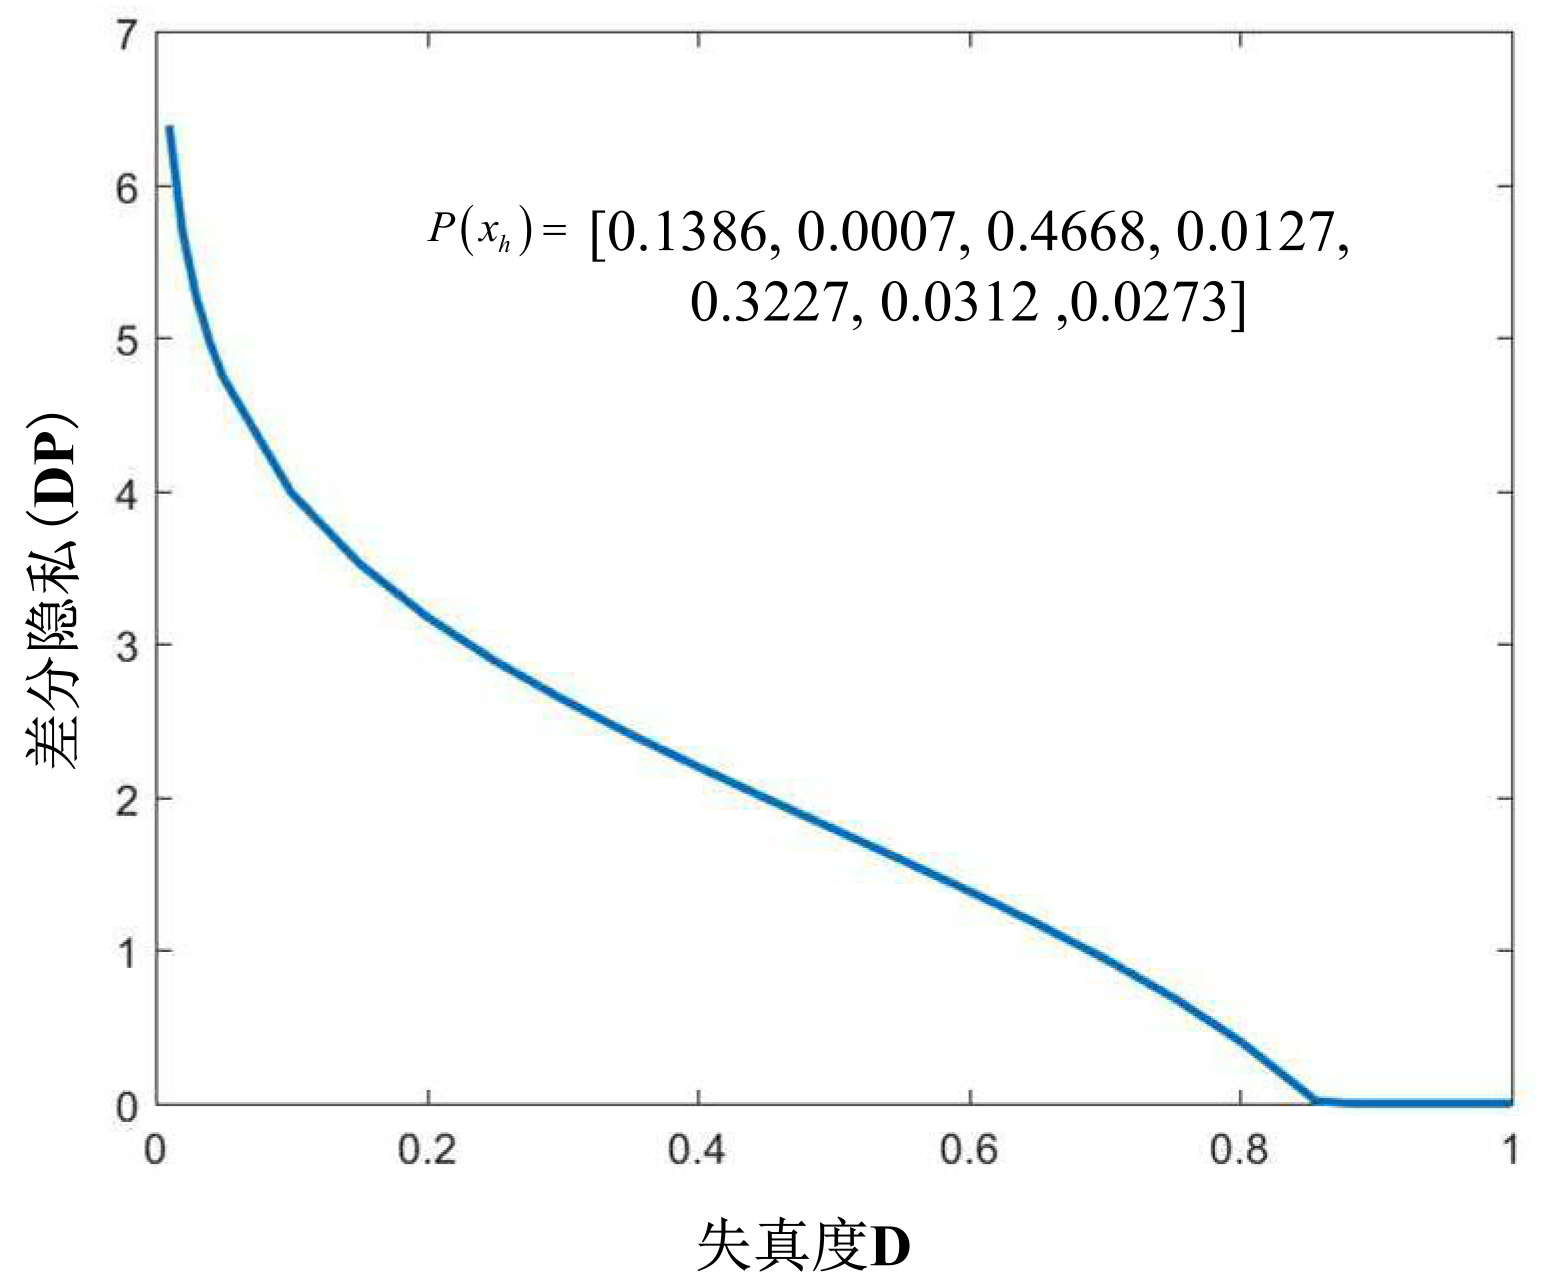
\includegraphics[width=8cm]{./figures/chapter03/Figure2.png}
		\caption{差分隐私预算参数与失真度关系}
		\label{fig:epsilon_distortion}
	\end{minipage}
	\begin{minipage}[t]{0.48\textwidth}
		\centering
		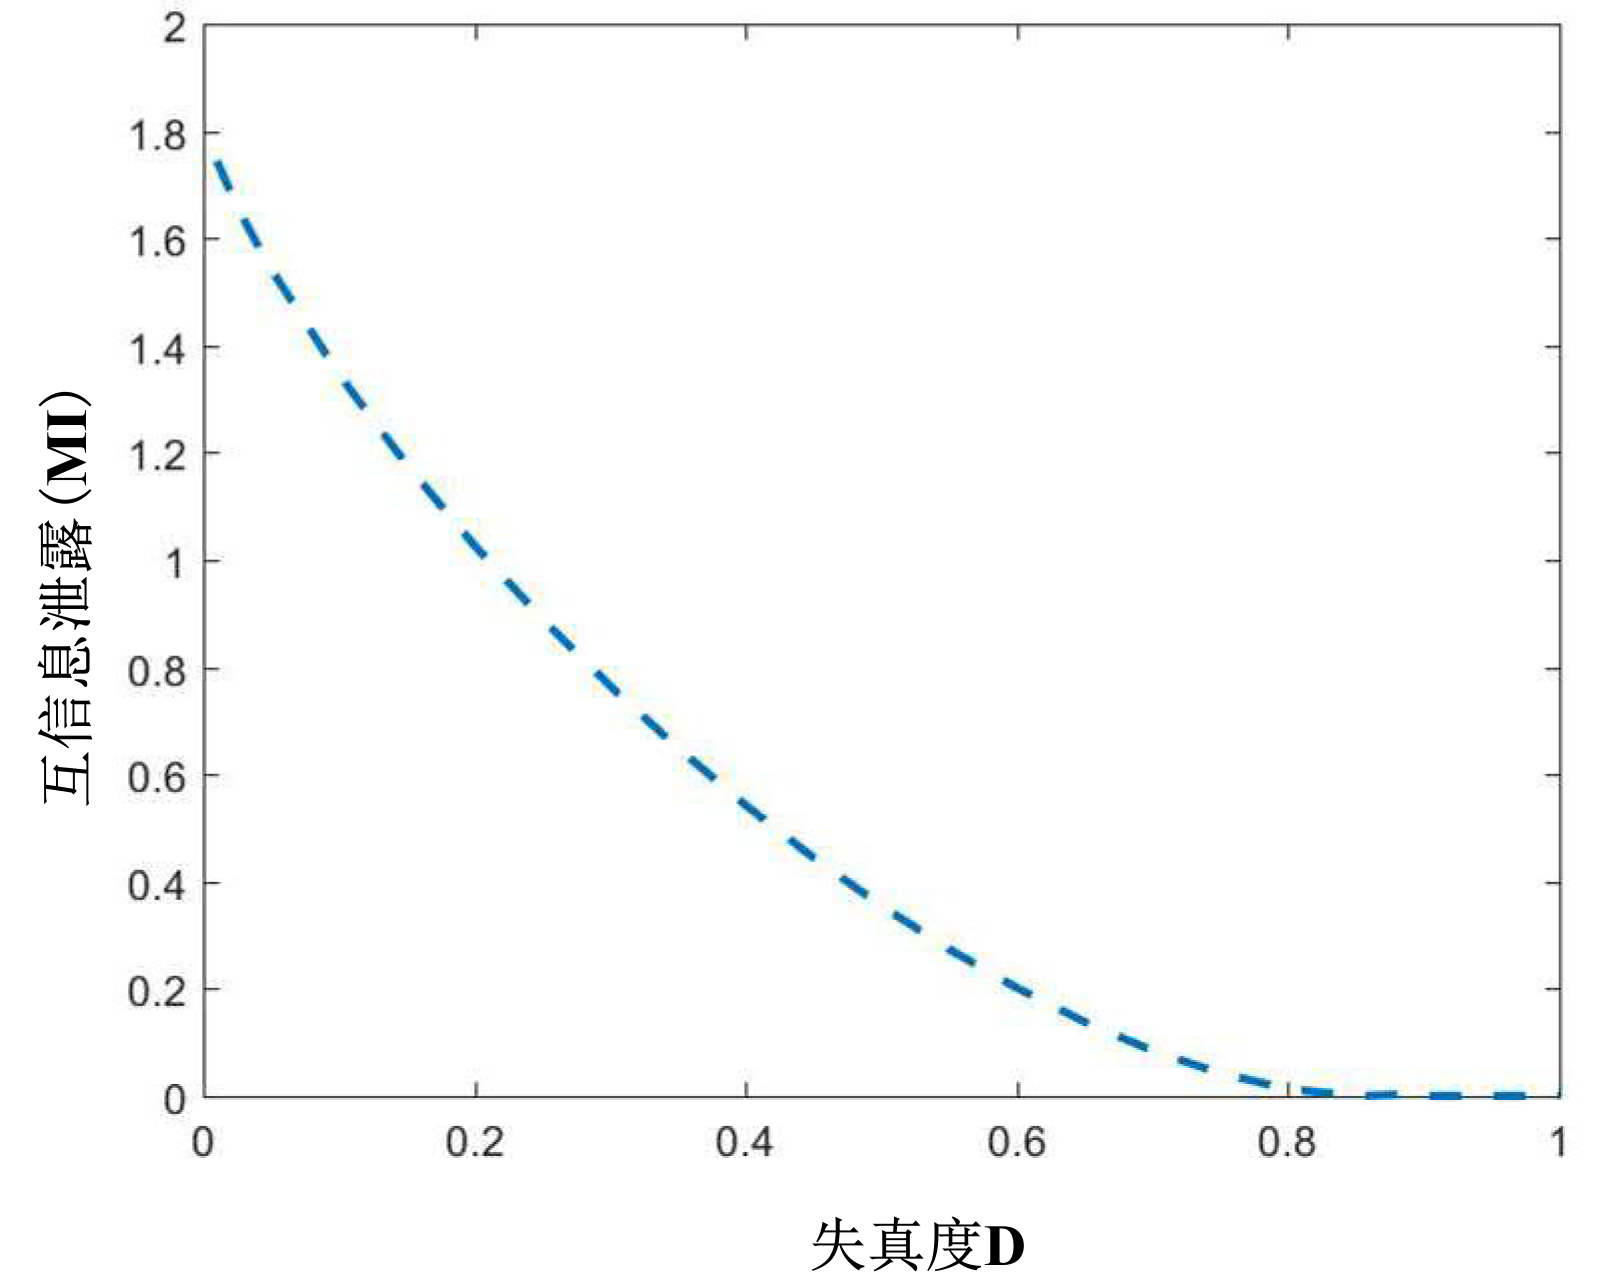
\includegraphics[width=8cm]{./figures/chapter03/Figure3.png}
		\caption{互信息隐私泄露与失真度关系}
		\label{fig:mi_distortion}
	\end{minipage}
\end{figure}

针对隐私敏感属性$X_h$,考虑文献\mycite{alvim2011differential}中的对称离散信道情形,敏感属性在字母表空间中的每个符号正确传输的概率为$1-D$,误差概率为$\frac{D}{6}$,则此时的信道条件概率矩阵是$(7\times7)$阶的对称矩阵。 首先,针对这样的隐私机制,依据公式\ref{eq:epsilon_2.10}计算信道条件概率满足的差分隐私参数,图\ref{fig:epsilon_distortion}给出了差分隐私$\epsilon^{*}$与失真程度的对应变化关系。其次,对于已知的信源分布和特定的隐私机制,采用互信息公式\ref{eq:entropty_2.10} 计算互信息隐私泄露与期望失真度$D$之间的变化关系,图\ref{fig:mi_distortion}的结果展示了$D\rightarrow 0$ 时,互信息隐私泄露量$I(X_h;\hat{X}_h)\rightarrow H(X_h)$,由此验证分析了信息熵度量方法的有效性。



针对数据关联的隐私问题,文献\mycite{sankar2013utility}依据联合概率表达类别型属性之间具有的相关性,而对服从高斯分布的两相关联数值型随机变量$X$和$Y$,均值为$0$,方差为$\sigma_{X}^{2}$和$\sigma_{Y}^{2}$,采用皮尔逊相关系数法$\rho_{XY}=\mathbb{E}[XY]/(\sigma_X,\sigma_Y)$量化两随机变量之间的相关度。 然而,皮尔逊相关系数法适用于量化两两变量总体满足或接近高斯分布的线性相关性,对于非线性关系和非数值文本相关性的测量存在着不足。对比与上述采用的方法,本章中互信息的分析方法具有以下优势:

(1) 首先,本章基于Shannon通信模型,建立差分隐私通信模型。随后,研究面向多维属性关联关系数据集发布,提出的信息熵度量模型及方法针对更具体的差分隐私保护机制。

(2) 其次,采用互信息量化多维属性之间关联的相关度,是对数值型变量线性相关性分析的推广与延伸。互信息相关性分析克服了应用于混合数值型和类别型属性的局限性,能够有效的表达复杂的相关型关系。

(3) 最后,基于样本观测数据分析属性关联度,设定阈值门限过滤属性伪相关的影响,并据此生成属性的关联依赖图。然后,将属性集合划分为隐私关联属性组和隐私敏感属性,依据相关度的互信息隐私泄露度量相较于主观的划分更有科学理论。

\section{本章小结}
本章基于Shannon基本通信模型,给出差分隐私通信模型及其信道数学模型。以此通信模型为基本出发点,构建了一种属性关联、元组记录独立同分布的离散无记忆信源的$n$次扩展信源。在此基础上,引入信息熵、条件熵、互信息量、失真函数等概念给出了隐私信源熵、隐私熵与隐私泄露风险、数据效用的基本度量模型及方法。进一步,针对多维属性关联的隐私度量问题,基于信息熵提出了面向关联属性的差分隐私信息熵度量模型及方法。首先,利用互信息相关性分析方法解决关联属性相关度量化问题。随后,基于相关度给出关联属性的图表示。进一步,基于差分隐私的信道模型、属性关联图中隐私泄露关键路径,借助马尔可夫理论分析了关联属性导致敏感信息的隐私泄露量。最后,以真实数据集上的实验给出所提出的信息熵度量模型及方法的量化过程及结果。本章是研究差分隐私信息论度量的基础工作,为后续基于隐私信息度量研究权衡隐私与效用均衡优化模型以及隐私机制设计奠定基础。

